
\section{Testing Setup}
\label{section: experimental setup - testing setup}

%     -[[ Hardware Setup ]]-
% - What exact chip do we use, what exact Kinect
% - What firmware do we run, and why
% - refer to the appendix with more in-depth info
% - 
% FMCW
The mmWave~radar used in this thesis is the IWR6843ISK by Texas~Instruments.
The radar requires firmware to run, a diverse variety of which are provided by Texas Instruments, for varying sensing tasks.
% The radar runs firmware, a variety of which are provided by TI, for various sensing tasks.
% This chip needs to run a specific firmware to work; TI provides a set of ready-made firmware, which differ slightly in what they provide to the end user.
The main firmware characteristics that are important to this thesis are the number of points generated, the signal-to-noise ratio, and the discriminative value of each point, for arm angle estimation.
% For this thesis, a "useful" point can tell you a lot about the position of a (semi-static) arm.
We chose the \textit{Mobile Tracker} firmware~\cite{ti_mmwave_firmware} as it meets those criteria.
% These criteria were met by the \textit{Mobile Tracker} firmware~\cite{ti_mmwave_firmware}. 
% For this reason, and the fact that the firmware aligned well with an interpretation method which was being explored at the time, this became the firmware of choice.
For a more detailed discussion of this firmware choice, see Appendix~\ref{appendix: configuration in detail}.
% Kinect
In addition to the mmWave Radar, a Kinect 2 was used to collect ground truth data.
The skeletal estimation was generated through a code base published by Kharche on GitHub~\cite{kharche2019skeletal}, which creates a smooth skeletal estimation and saves it, along with timestamps, to a CSV file.
This skeletal estimation was transformed into an arm angle estimation by calculating the angle of the vector going from the \textit{neck keypoint} to either \textit{wrist keypoint}, with regards to the down vector, see \cref{figure: kinect angle}.

\begin{figure}[!htb]
    \centering
    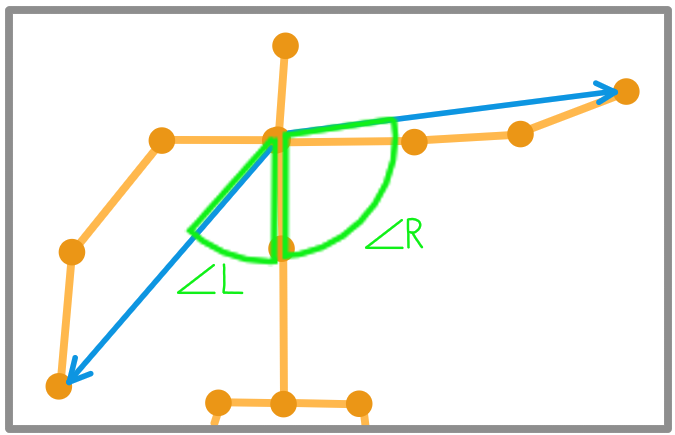
\includegraphics[width=0.5\linewidth]{figures/internal data/gt angle calculation diagram.png}
    \caption{Skeletal estimation into Arm Angle estimation visualisation.}
    \label{figure: kinect angle}
\end{figure}

\begin{figure}[!htb]
    \centering
    \begin{subfigure}{0.45\textwidth}
       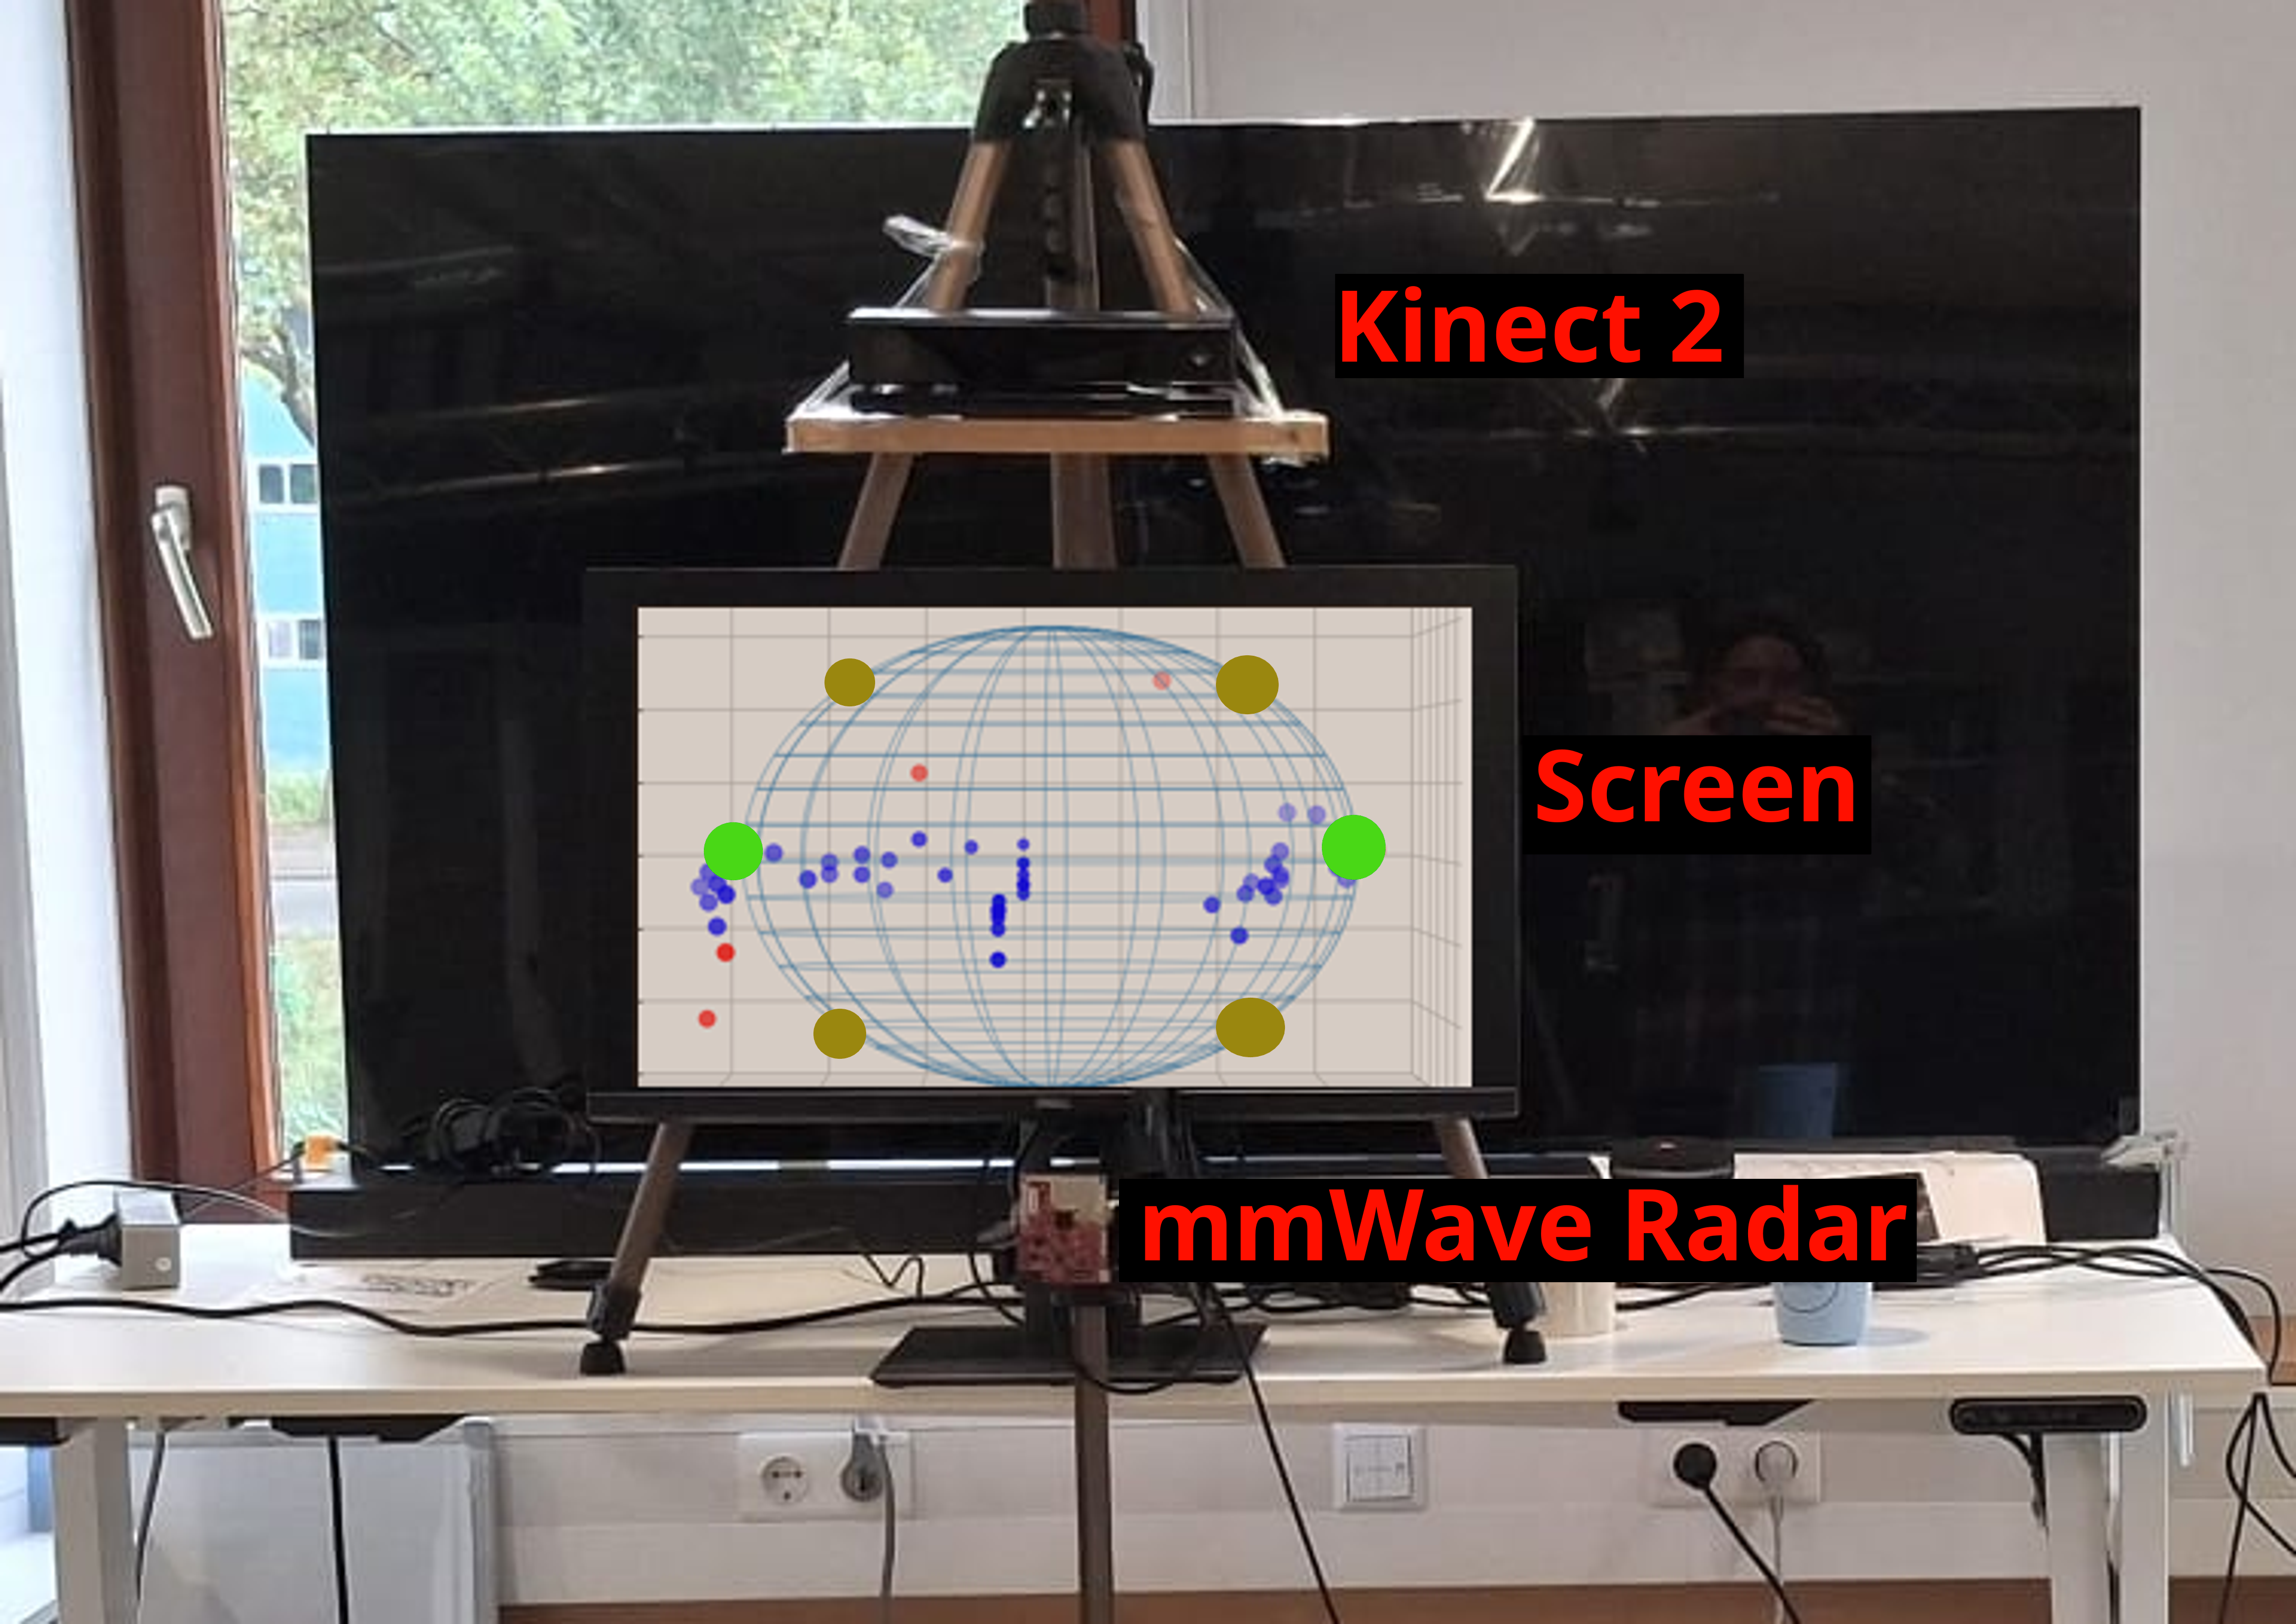
\includegraphics[width=1\textwidth]{figures/experimental setup/sensor view edit.png}
       \caption{User view}
    \label{figure: testing environment - user view}
    \end{subfigure}
    \hfill
    \begin{subfigure}{0.45\textwidth}
       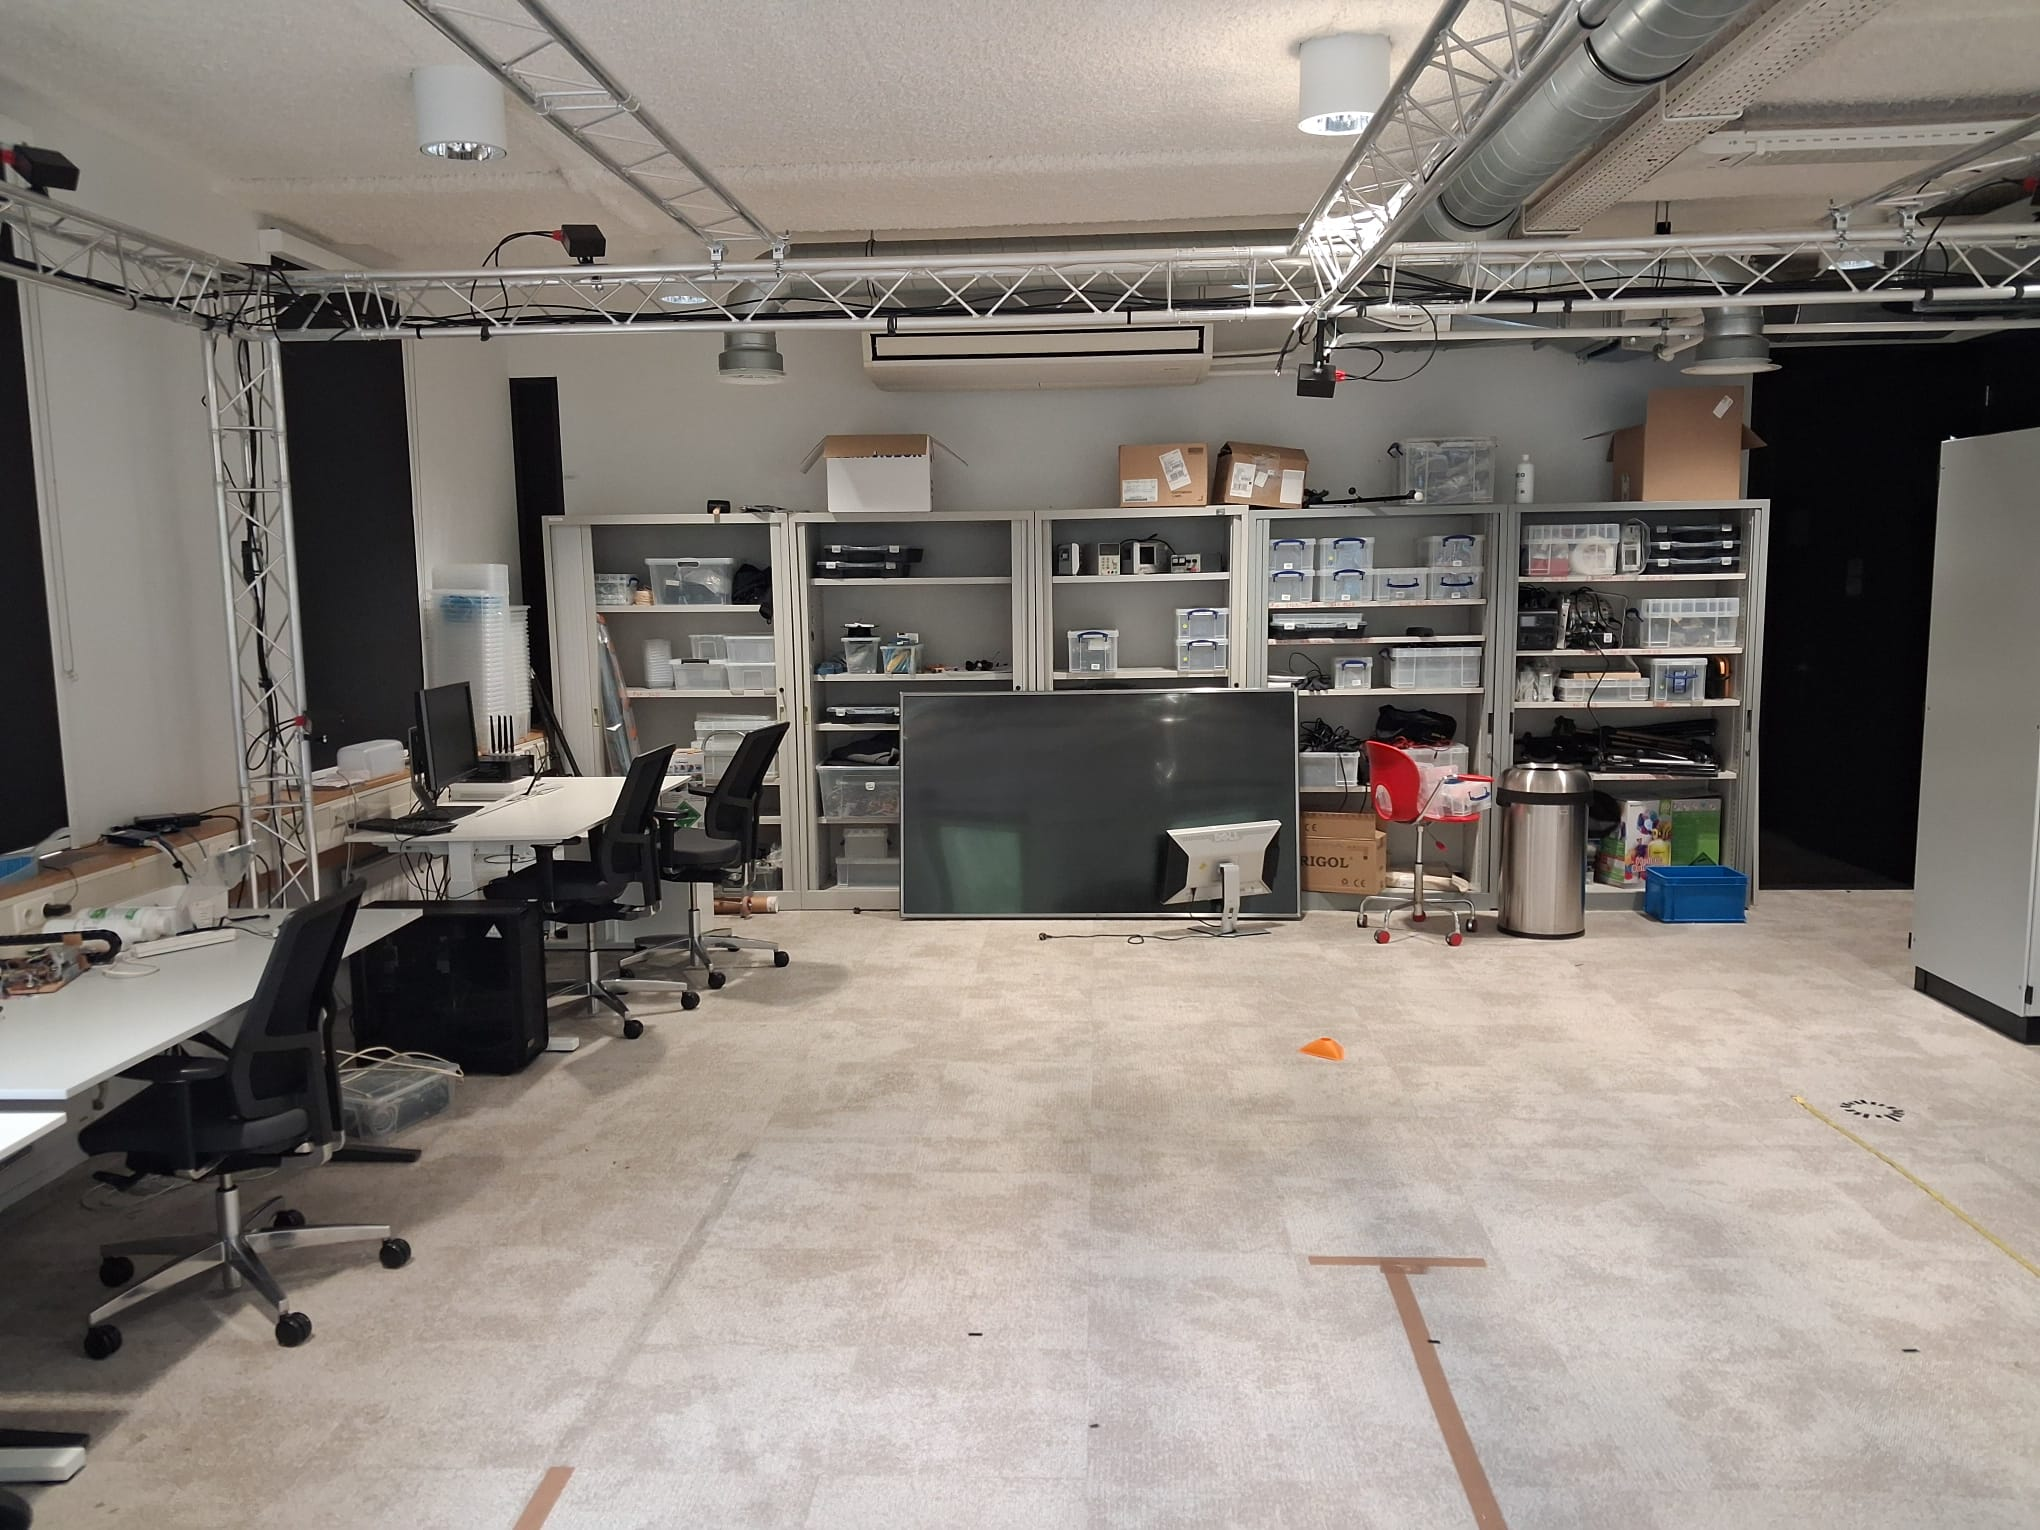
\includegraphics[width=1\textwidth]{figures/experimental setup/room_view.jpeg}
       \caption{View from the Sensor's perspective}
       \label{figure: testing environment - sensor view}
    \end{subfigure}
    \caption{The testing environment, providing the user view (a) and the sensor's perspective (b).}
    \label{figure: testing environment}
\end{figure}

%     -[[ Physical setup ]]-
% - What does the room look like
%   - Where was the sensor
%   - Where was the user
% - What effect could the room setup have
% - 
The experiments are performed in a large open room ($7 \times 10$~m). 
The mmWave~radar was mounted at a height of 125~cm and was tilted upwards at an angle of $5\degree$.
The Kinect was mounted at a height of 175~cm with an angle of $5\degree$ downwards.
The user could see a real-time visualisation of the incoming point cloud, as well as the current arm angle estimation on a screen in front of them, as shown in \cref{figure: testing environment - user view}.
% A screen was also present, on which the user could see their currently predicted zones, and the incoming point clouds.
The user was standing at a distance of 2 meters from the sensors.
Appendix \ref{appendix: experimental setup} shows the experimental setup in detail.
A large and open room was used, see \cref{figure: testing environment - sensor view}, which meant that back wall reflections were spatially distinct from the user.
This resulted in point clouds with relatively little noise, producing a relatively high-quality dataset.
% \ednote{Info about the back wall is not needed and only confusing}
% The back wall was also broken up with open shelving, diffusing any potential backscatter.
% % which should've scattered the incoming millimeter waves, as opposed to reflecting them.
% The large screen at the end of the room was angled upwards, reflecting the mmWaves away from, rather than back at, the radar.
% % The large screen present was angled upwards, and would've thus not reflected the signal to the mmWave sensor.
% These factors resulted in the mmWave radar producing point clouds with relatively little noise in this room, which in turn reduced the need for aggressive noise reduction, creating a higher-quality dataset.
% % meant that the noise reduction algorithms did not have to be tuned as much.



%     -[[ Testing procedures]]-
% - How was the user informed
% - What were they asked to do
% - How did we provide feedback
% - Refer to the appendix for more in-depth info
% - 

Six users took part in this experiment.
For each user, we collected between 4 and 7 recordings; the average duration of a recording is 140 seconds.
Each recording consists of two distinct parts: the \textit{calibration} part, and the \textit{interpretation} part.
The \textit{calibration} had an average duration of 20 seconds, during which the user moved their arms up and down. % along their body.
The remainder of the recording is part of the \textit{interpretation}, and has an average duration of 120 seconds.
During the \textit{interpretation}, the user moves their arms to a specific position and holds the position for a few seconds before moving their arms to the next position.
% The whole experiment consisted of between 4 and 7 recordings per user.
% During these recordings, the users
% , took between 20 and 40 minutes.
During the recordings, both the mmWave radar point cloud and a skeletal estimation produced by the Kinect 2 were recorded.
The Kinect 2 recorded a video channel, but this video channel was only used to create the skeletal estimate and was never saved.
While in use, the system produced musical notes in accordance with the pose that the system predicted at that given time.
The users were given a consent form before the experiment, and were allowed to drop out of the experiment at any point.
For privacy reasons, we chose only to record the height and arm span of the users, and no other information, see Appendix~\ref{appendix: user information}.
Before the experiment took place, we informed the users of how the system worked and what was expected of them through an explanatory PDF (see Appendix~\ref{appendix: user explanation}).
The specific actions the users performed are discussed in \cref{section: experimental setup - dataset}.

% \ednote{Briefly explain the general testing situation, "how many people did we have", "how long roughly did each test take", and also "what data do we record", and the fact that the users hear the music output.\\ Briefly mention (and forward references to explanation) how many standard recordings and free play people had, and roughly how long they took.}
% \ednote{Specify that we did not make any user interviews, briefly mention our privacy concern stuff.}
 % Users were informed of how the system worked and what they were expected to do through an explanatory PDF (see Appendix~\ref{appendix: user explanation}).
% The specific actions the users performed will be discussed in \cref{section: experimental setup - dataset}.
% \ednote{This "advice part" can mostly be skipped/removed.}
% After each recording, the researcher provided some guidance to the user about how to best use the system, based on the user error observed in the previous recording.
% Common advice included keeping consistent micro-movements in the hands to increase the point cloud stability and density in those regions.
% Furthermore, a more precise specification of the exact \textit{spatial regions} which correlated to a specific \textit{arm position} ("low", "middle", or "high") was also often given as advice.
% % Commonly given advice was to wave their hands, or do "jazz hands", as well as informing the user where the optimal "zone positions" are (for low, mid, high).
% A more detailed overview of the provided feedback, along with notes of the user performance, can be found in Appendix \ref{appendix: experiment notes}.


%     -[[ ]]-
% - 
% - 
% - 
%     -[[ ]]-

% Double separation line and spacing
% \vspace{2em}
% \hrule
% \vspace{0.2em}
% \hrule
% \vspace{2em}

%     [[ Hardware setup (chip, firmware, config ]]
% Describe the chip we used, the config we used on that chip, the reason for that choice, the specific config used.
% Also, describe the method for ground truth collection.

% The mmWave radar used for this thesis was the IWR6843ISK by Texas Instruments.
% The firmware which is used on this chip is the \textit{Mobile Tracker} firmware \cite{ti_mmwave_firmware}, in part chosen due to it producing a reasonable number of relatively representative points, and in part due to legacy reasons, which are further discussed in Appendix \ref{appendix: configuration in detail}.
% Next to this, a Microsoft Kinect 2 was used to collect the ground truth.
% To get a skeletal estimation from the Kinect, a code base by \citeauthor{kharche2019skeletal}\cite{kharche2019skeletal} was used.
% This code base could record the skeletal estimation produced by the Kinect to a CSV file, with timestamps for each frame, making it a good choice for the ground truth.


%     [[ Hardware setup p2. ]]
% Discuss the specific firmware used, what the advantages and disadvantages are, and what other options we might have had.
% -- [ SKIP ] -- 

%     [[ Environment setup (mounting, space) ]]
% Describe the room in which the tests were held, describe the positions for the various sensors, as well as the position of the user
% Use photos, specify measurements/distances

% [[ Testing procedure ]]
% Describe the testing procedure.
% Describe the types of data that were collected and why,
% Describe the way in which the user was guided.

% Explain the type of room we took measurements in and why, also describe the sensors we use (fmcw + kinect)

% Describe the test setup specifically, use photos and specify measurements (user stood at a distance of 2m)

% Explain the testing procedure, what did we tell the users?